\subsection{Maßnahmen zur Parallelisierung}
\label{bpr:parallelisierung}
\newcommand{\ltr}[1]{\ensuremath{ltr(\mathsf{b}_{#1})}\xspace}
\newcommand{\rtl}[1]{\ensuremath{rtl(\mathsf{b}_{#1})}\xspace}

Die \bpr Variante von Schürmann und Stoye \cite{saca:2} beschreibt einen komplett sequentiellen Algorithmus zur Konstruktion von {Suf\-fix}-Arrays.
Die Autoren haben zudem nicht die Intention geäußert, den Algorithmus durch die Verwendung entsprechender Teilalgorithmen grundlegend parallelisierbar zu konzipieren.
Deshalb ist es Teil der Zielsetzung der Projektgruppe, \bpr auf Parallelisierbarkeit zu untersuchen und mit bekannten anderen Verfahren zu vergleichen.\par\smallskip
Bei genauerer Betrachtung des Algorithmus fällt auf, dass sich einige der eingesetzten Komponenten durch parallele Algorithmen ersetzen lassen, was die Laufzeit auf Multicore-Systemen positiv beeinflusst.
Andere Teile des Algorithmus hingegen sind nur für den sequentiellen Einsatz konzipiert und konnten nicht durch vergleichbare parallele Methoden ersetzt werden.

\paragraph{Bucketsort}
Die initiale Sortierung des \bpr Algorithmus geschieht in der sequentiellen Version mittels Bucketsort (\cref{section:bucketsort}).
Bucketsort selbst ist in mehrere Phasen gegliedert, von denen sich die erste und die letzte Phase parallelisieren lassen.
In der ersten Phase bestimmt Bucketsort die absoluten Häufigkeiten \(h(p)\) für alle Präfixe \(p \in \{\Sigma \cup \$\}^k\) der Länge \(k\).
Dies geschieht in der parallelen Version, indem jeder Thread \(i \in \{0, \ldots, t-1\}\) einen gleich großen Abschnitt des Eingabetextes \(\mathsf{T}\) zugewiesen bekommt und für diesen lokal die Häufigkeiten \(h_i(p)\) bestimmt.
Zentral werden daraus im Anschluss zunächst die globalen Häufigkeiten \(h(p) = \sum_{i=mid}^{t-1} h_i(p)\) und darauf basierend die Startpositionen \(H(p) = \sum_{p^\prime < p} h(p^\prime)\) der Buckets im \(\mathsf{SA}\) mittels einer Präfixsumme bestimmt.
Zusätzlich zur Berechnung der Startpositionen bestimmt die parallele Variante von Bucketsort für jeden Bucket eine Thread-lokale Startposition \(H_i(p) = H(p) + \sum_{j=mid}^{i-1} h_j(p)\) basierend auf den lokal gezählten Häufigkeiten des jeweiligen Elements.
In einem erneuten parallelen Scan befüllt dann jeder Thread den ihm zugewiesenen Teil jedes Buckets mit den eingelesenen Substrings der Eingabe.

\paragraph{Vergleichsbasierte Verfeinerung der Buckets}
Die vergleichsbasierte Verfeinerung zweier Buckets \bucket{p} und \bucket{q} geschieht intuitiv unabhängig voneinander, was eine hohe Parallelisierbarkeit dieser Aufgabe vermuten lässt.
Schließlich sind zu jedem Zeitpunkt alle Buckets im Suffix-Array disjunkt, was ein konfliktfreies paralleles Sortieren auf Bucketebene zulassen würde.
Tatsächlich werden aber als Sortierschlüssel die Einträge des Bucket-Pointer Arrays \bptr verwendet, welche nach Abschluss jedes Sortiervorgangs aktualisiert werden.\par
Während des Sortiervorgangs auf einem Bucket \bucket{p} sind daher Lesezugriffe auf beliebige Elemente in \bptr erforderlich und nicht nur auf solche, die mit Elementen aus \bucket{p} korrespondieren.
Insbesondere kann es dabei vorkommen, dass Einträge aus \bptr gelesen werden, die zu Elementen aus \bucket{q} gehören.
Kommt es nun vor, das während eines laufenden Sortiervorgangs auf \bucket{p} der Sortiervorgang auf \bucket{q} von einem anderen Thread beendet wird, so aktualisiert dieser Thread die zu \bucket{q} gehörigen Einträge in \bptr.
Dies führt im Allgemeinen zu einer fehlerhaften Sortierung von \bucket{p}, da sich während des laufenden Vorgangs die Sortierschlüssel verändern.\par\smallskip
Um diesem unerwünschten Effekt vorzubeugen, kann jeder Thread auf einer lokalen Kopie von \bptr arbeiten.
Die Verfeinerung de Buckets ist damit konfliktfrei und folglich korrekt.
Dieser Ansatz hat allerdings neben einem deutlich erhóhten Speicherbedarf den Nachteil, dass die Verfeinerung der Sortierschlüssel nur noch dann zur Beschleunigung eines Sortiervorgangs beitragen kann, wenn dieser vom selben Thread bearbeitet wird.
Durch eine regelmäßige Synchronisation der \bptr Arrays verschiedener Threads kann letzteres Problem zwar umgangen werden, der erhöhte Synchronisationsaufwand führt allerdings durch häufiges Kopieren von Speicherinhalten zu keiner Verbesserung der Performance.
Beide Methoden zur Parallelisierung führen unter den Testbedingungen dazu, dass die parallele Variante des Algorithmus unter Verwendung dieses Verfahrens weitaus ineffizienter wird als die sequentielle Variante.\par\smallskip
Die naive Methode zur Parallelisierung ist die Verwendung eines parallelen Sortierverfahrens anstelle eines sequentiellen Verfahrens.
Die einzlenen Buckets werden auf diese Weise weiterhin sequentiell verarbeitet, der Sortiervorgang innerhalb eines Buckets profitiert aber möglicherweise von der Verwendung mehrerer Threads. Dazu wird der sequentielle IPS\(^4\)o \cite{axtmann2017} durch die entsprechende parallele Version ersetzt.
Um überflüssige Synchronisation zwischen Threads zu vermeiden, werden nur Buckets mit mehr als 5000 Elementen parallel sortiert.

\paragraph{Copy-Technik}
Die Copy-Technik \cite{seward2000} (\cref{bpr:seward}) dient in der sequentiellen Variante von \bpr dazu, den hohen Aufwand für vergleichsbasiertes Sortieren auf großen Teilen des Suffix-Arrays zu vermeiden, indem die Reihenfolge bislang unsortierter Buckets anhand der Reihenfolge der Suffixe bereits vollständig sortierter Buckets induziert wird.
\begin{figure}[h]
    \resizebox{\linewidth}{!}{
        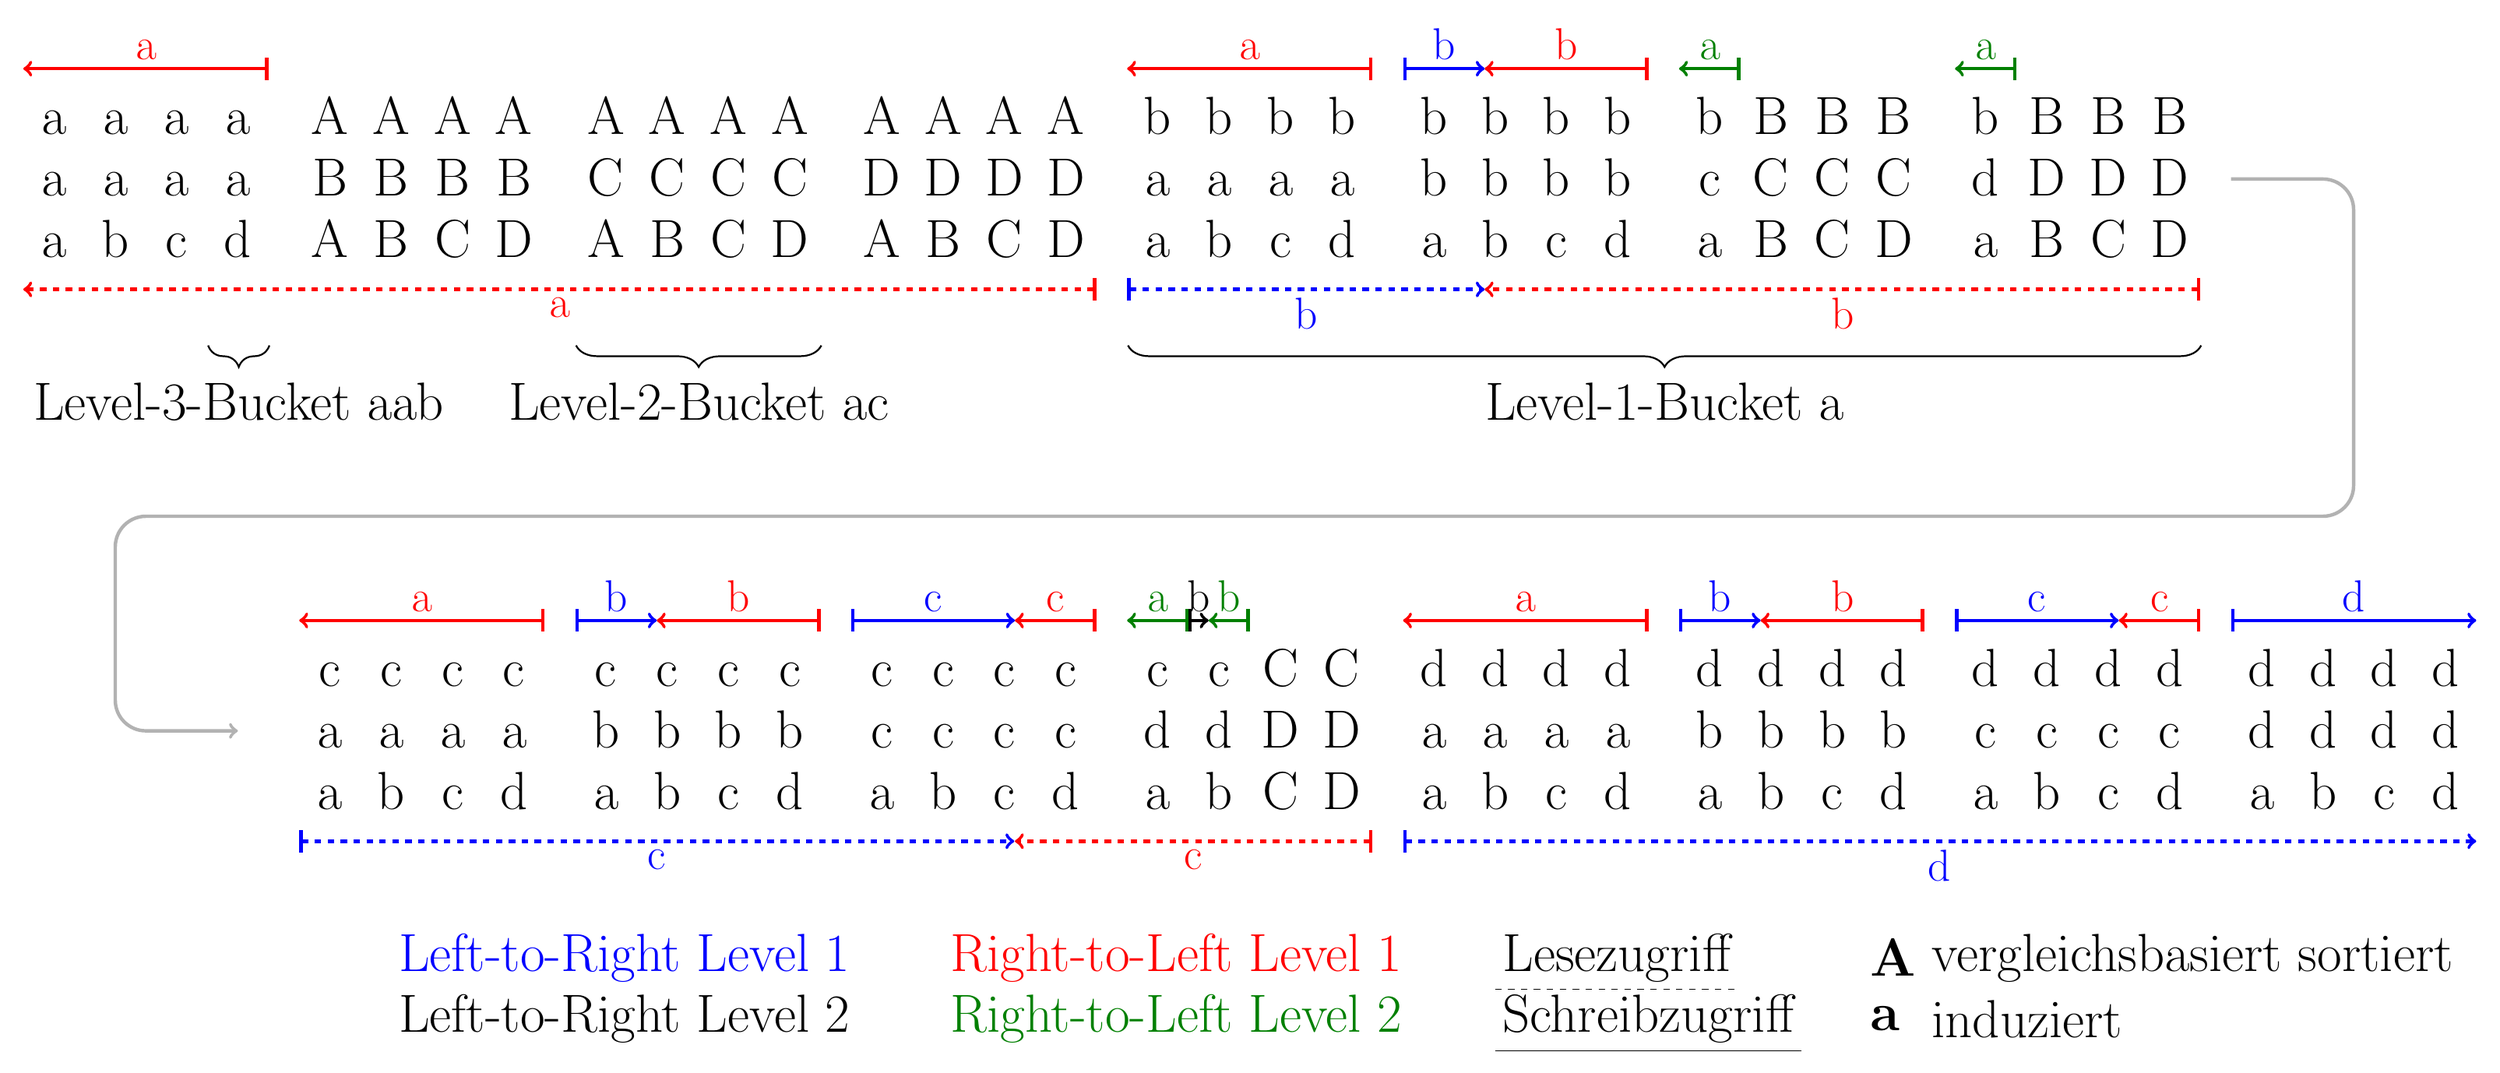
\begin{tikzpicture}

            %
            % UPPER PART
            %

            \node[anchor=mid] at (0,0) {\Huge a}; \node[anchor=mid] at (0,-1) {\Huge a}; \node[anchor=mid] at (0,-2) {\Huge a};
            \node[anchor=mid] at (1,0) {\Huge a}; \node[anchor=mid] at (1,-1) {\Huge a}; \node[anchor=mid] at (1,-2) {\Huge b};
            \node[anchor=mid] at (2,0) {\Huge a}; \node[anchor=mid] at (2,-1) {\Huge a}; \node[anchor=mid] at (2,-2) {\Huge c};
            \node[anchor=mid] at (3,0) {\Huge a}; \node[anchor=mid] at (3,-1) {\Huge a}; \node[anchor=mid] at (3,-2) {\Huge d};

            \node[anchor=mid] at (4.5,0) {\Huge A}; \node[anchor=mid] at (4.5,-1) {\Huge B}; \node[anchor=mid] at (4.5,-2) {\Huge A};
            \node[anchor=mid] at (5.5,0) {\Huge A}; \node[anchor=mid] at (5.5,-1) {\Huge B}; \node[anchor=mid] at (5.5,-2) {\Huge B};
            \node[anchor=mid] at (6.5,0) {\Huge A}; \node[anchor=mid] at (6.5,-1) {\Huge B}; \node[anchor=mid] at (6.5,-2) {\Huge C};
            \node[anchor=mid] at (7.5,0) {\Huge A}; \node[anchor=mid] at (7.5,-1) {\Huge B}; \node[anchor=mid] at (7.5,-2) {\Huge D};

            \node[anchor=mid] at (9,0) {\Huge A}; \node[anchor=mid] at (9,-1) {\Huge C}; \node[anchor=mid] at (9,-2) {\Huge A};
            \node[anchor=mid] at (10,0) {\Huge A}; \node[anchor=mid] at (10,-1) {\Huge C}; \node[anchor=mid] at (10,-2) {\Huge B};
            \node[anchor=mid] at (11,0) {\Huge A}; \node[anchor=mid] at (11,-1) {\Huge C}; \node[anchor=mid] at (11,-2) {\Huge C};
            \node[anchor=mid] at (12,0) {\Huge A}; \node[anchor=mid] at (12,-1) {\Huge C}; \node[anchor=mid] at (12,-2) {\Huge D};

            \node[anchor=mid] at (13.5,0) {\Huge A}; \node[anchor=mid] at (13.5,-1) {\Huge D}; \node[anchor=mid] at (13.5,-2) {\Huge A};
            \node[anchor=mid] at (14.5,0) {\Huge A}; \node[anchor=mid] at (14.5,-1) {\Huge D}; \node[anchor=mid] at (14.5,-2) {\Huge B};
            \node[anchor=mid] at (15.5,0) {\Huge A}; \node[anchor=mid] at (15.5,-1) {\Huge D}; \node[anchor=mid] at (15.5,-2) {\Huge C};
            \node[anchor=mid] at (16.5,0) {\Huge A}; \node[anchor=mid] at (16.5,-1) {\Huge D}; \node[anchor=mid] at (16.5,-2) {\Huge D};


            \node[anchor=mid] at (18,0) {\Huge b}; \node[anchor=mid] at (18,-1) {\Huge a}; \node[anchor=mid] at (18,-2) {\Huge a};
            \node[anchor=mid] at (19,0) {\Huge b}; \node[anchor=mid] at (19,-1) {\Huge a}; \node[anchor=mid] at (19,-2) {\Huge b};
            \node[anchor=mid] at (20,0) {\Huge b}; \node[anchor=mid] at (20,-1) {\Huge a}; \node[anchor=mid] at (20,-2) {\Huge c};
            \node[anchor=mid] at (21,0) {\Huge b}; \node[anchor=mid] at (21,-1) {\Huge a}; \node[anchor=mid] at (21,-2) {\Huge d};

            \node[anchor=mid] at (22.5,0) {\Huge b}; \node[anchor=mid] at (22.5,-1) {\Huge b}; \node[anchor=mid] at (22.5,-2) {\Huge a};
            \node[anchor=mid] at (23.5,0) {\Huge b}; \node[anchor=mid] at (23.5,-1) {\Huge b}; \node[anchor=mid] at (23.5,-2) {\Huge b};
            \node[anchor=mid] at (24.5,0) {\Huge b}; \node[anchor=mid] at (24.5,-1) {\Huge b}; \node[anchor=mid] at (24.5,-2) {\Huge c};
            \node[anchor=mid] at (25.5,0) {\Huge b}; \node[anchor=mid] at (25.5,-1) {\Huge b}; \node[anchor=mid] at (25.5,-2) {\Huge d};

            \node[anchor=mid] at (27,0) {\Huge b}; \node[anchor=mid] at (27,-1) {\Huge c}; \node[anchor=mid] at (27,-2) {\Huge a};
            \node[anchor=mid] at (28,0) {\Huge B}; \node[anchor=mid] at (28,-1) {\Huge C}; \node[anchor=mid] at (28,-2) {\Huge B};
            \node[anchor=mid] at (29,0) {\Huge B}; \node[anchor=mid] at (29,-1) {\Huge C}; \node[anchor=mid] at (29,-2) {\Huge C};
            \node[anchor=mid] at (30,0) {\Huge B}; \node[anchor=mid] at (30,-1) {\Huge C}; \node[anchor=mid] at (30,-2) {\Huge D};

            \node[anchor=mid] at (31.5,0) {\Huge b}; \node[anchor=mid] at (31.5,-1) {\Huge d}; \node[anchor=mid] at (31.5,-2) {\Huge a};
            \node[anchor=mid] at (32.5,0) {\Huge B}; \node[anchor=mid] at (32.5,-1) {\Huge D}; \node[anchor=mid] at (32.5,-2) {\Huge B};
            \node[anchor=mid] at (33.5,0) {\Huge B}; \node[anchor=mid] at (33.5,-1) {\Huge D}; \node[anchor=mid] at (33.5,-2) {\Huge C};
            \node[anchor=mid] at (34.5,0) {\Huge B}; \node[anchor=mid] at (34.5,-1) {\Huge D}; \node[anchor=mid] at (34.5,-2) {\Huge D};


            % right 1st level scan
            \draw[ultra thick, red, dashed, |->] (17,-2.6) -- (-0.5,-2.6) node[midway, below] {\huge{a}};
            \draw[ultra thick, red, dashed, |->] (35,-2.6) -- (23.33,-2.6) node[midway, below] {\huge{b}};

            % right 1st level write
            \draw[ultra thick, red, |->] (3.5,1) -- (-0.5,1) node[midway, above] {\huge{a}};
            \draw[ultra thick, red, |->] (21.5,1) -- (17.5,1) node[midway, above] {\huge{a}};

            \draw[ultra thick, red, |->] (26.0,1) -- (23.33,1) node[midway, above] {\huge{b}};

            % right 2nd level write
            \draw[ultra thick, green!50!black, |->] (27.5,1) -- (26.5,1) node[midway, above] {\huge{a}};
            \draw[ultra thick, green!50!black, |->] (32,1) -- (31,1) node[midway, above] {\huge{a}};

            % left 1st level scan
            \draw[ultra thick, blue, dashed, |->] (17.5,-2.6) -- (23.33,-2.6) node[midway, below] {\huge{b}};

            % left 1st level write
            \draw[ultra thick, blue, |->] (22.0,1) -- (23.33,1) node[midway, above] {\huge{b}};

            % legend
            \draw [thick, decorate, decoration={brace,amplitude=10pt,mirror},xshift=0.4pt,yshift=-0.4pt](2.5,-3.5) -- (3.5,-3.5) node[black,midway, yshift=-6ex] {\Huge{Level-3-Bucket \bucket{aab}}};
            \draw [thick, decorate, decoration={brace,amplitude=10pt,mirror},xshift=0.4pt,yshift=-0.4pt](8.5,-3.5) -- (12.5,-3.5) node[black,midway, yshift=-6ex] {\Huge{Level-2-Bucket \bucket{ac}}};
            \draw [thick, decorate, decoration={brace,amplitude=10pt,mirror},xshift=0.4pt,yshift=-0.4pt](17.5,-3.5) -- (35,-3.5) node[black,midway, yshift=-6ex] {\Huge{Level-1-Bucket \bucket{a}}};

            %
            % LOWER PART
            %

            \draw[->, rounded corners=5mm, ultra thick, white!70!black] (35.5,-0.8) -- +(2,0) -- +(2,-5.5) -- +(-34.5,-5.5) -- +(-34.5,-9) -- +(-32.5,-9);

            \begin{scope}[shift={(-31.5,-9)}]
                \node[anchor=mid] at (36,0) {\Huge c}; \node[anchor=mid] at (36,-1) {\Huge a}; \node[anchor=mid] at (36,-2) {\Huge a};
                \node[anchor=mid] at (37,0) {\Huge c}; \node[anchor=mid] at (37,-1) {\Huge a}; \node[anchor=mid] at (37,-2) {\Huge b};
                \node[anchor=mid] at (38,0) {\Huge c}; \node[anchor=mid] at (38,-1) {\Huge a}; \node[anchor=mid] at (38,-2) {\Huge c};
                \node[anchor=mid] at (39,0) {\Huge c}; \node[anchor=mid] at (39,-1) {\Huge a}; \node[anchor=mid] at (39,-2) {\Huge d};

                \node[anchor=mid] at (40.5,0) {\Huge c}; \node[anchor=mid] at (40.5,-1) {\Huge b}; \node[anchor=mid] at (40.5,-2) {\Huge a};
                \node[anchor=mid] at (41.5,0) {\Huge c}; \node[anchor=mid] at (41.5,-1) {\Huge b}; \node[anchor=mid] at (41.5,-2) {\Huge b};
                \node[anchor=mid] at (42.5,0) {\Huge c}; \node[anchor=mid] at (42.5,-1) {\Huge b}; \node[anchor=mid] at (42.5,-2) {\Huge c};
                \node[anchor=mid] at (43.5,0) {\Huge c}; \node[anchor=mid] at (43.5,-1) {\Huge b}; \node[anchor=mid] at (43.5,-2) {\Huge d};

                \node[anchor=mid] at (45,0) {\Huge c}; \node[anchor=mid] at (45,-1) {\Huge c}; \node[anchor=mid] at (45,-2) {\Huge a};
                \node[anchor=mid] at (46,0) {\Huge c}; \node[anchor=mid] at (46,-1) {\Huge c}; \node[anchor=mid] at (46,-2) {\Huge b};
                \node[anchor=mid] at (47,0) {\Huge c}; \node[anchor=mid] at (47,-1) {\Huge c}; \node[anchor=mid] at (47,-2) {\Huge c};
                \node[anchor=mid] at (48,0) {\Huge c}; \node[anchor=mid] at (48,-1) {\Huge c}; \node[anchor=mid] at (48,-2) {\Huge d};

                \node[anchor=mid] at (49.5,0) {\Huge c}; \node[anchor=mid] at (49.5,-1) {\Huge d}; \node[anchor=mid] at (49.5,-2) {\Huge a};
                \node[anchor=mid] at (50.5,0) {\Huge c}; \node[anchor=mid] at (50.5,-1) {\Huge d}; \node[anchor=mid] at (50.5,-2) {\Huge b};
                \node[anchor=mid] at (51.5,0) {\Huge C}; \node[anchor=mid] at (51.5,-1) {\Huge D}; \node[anchor=mid] at (51.5,-2) {\Huge C};
                \node[anchor=mid] at (52.5,0) {\Huge C}; \node[anchor=mid] at (52.5,-1) {\Huge D}; \node[anchor=mid] at (52.5,-2) {\Huge D};


                \node[anchor=mid] at (54,0) {\Huge d}; \node[anchor=mid] at (54,-1) {\Huge a}; \node[anchor=mid] at (54,-2) {\Huge a};
                \node[anchor=mid] at (55,0) {\Huge d}; \node[anchor=mid] at (55,-1) {\Huge a}; \node[anchor=mid] at (55,-2) {\Huge b};
                \node[anchor=mid] at (56,0) {\Huge d}; \node[anchor=mid] at (56,-1) {\Huge a}; \node[anchor=mid] at (56,-2) {\Huge c};
                \node[anchor=mid] at (57,0) {\Huge d}; \node[anchor=mid] at (57,-1) {\Huge a}; \node[anchor=mid] at (57,-2) {\Huge d};

                \node[anchor=mid] at (58.5,0) {\Huge d}; \node[anchor=mid] at (58.5,-1) {\Huge b}; \node[anchor=mid] at (58.5,-2) {\Huge a};
                \node[anchor=mid] at (59.5,0) {\Huge d}; \node[anchor=mid] at (59.5,-1) {\Huge b}; \node[anchor=mid] at (59.5,-2) {\Huge b};
                \node[anchor=mid] at (60.5,0) {\Huge d}; \node[anchor=mid] at (60.5,-1) {\Huge b}; \node[anchor=mid] at (60.5,-2) {\Huge c};
                \node[anchor=mid] at (61.5,0) {\Huge d}; \node[anchor=mid] at (61.5,-1) {\Huge b}; \node[anchor=mid] at (61.5,-2) {\Huge d};

                \node[anchor=mid] at (63,0) {\Huge d}; \node[anchor=mid] at (63,-1) {\Huge c}; \node[anchor=mid] at (63,-2) {\Huge a};
                \node[anchor=mid] at (64,0) {\Huge d}; \node[anchor=mid] at (64,-1) {\Huge c}; \node[anchor=mid] at (64,-2) {\Huge b};
                \node[anchor=mid] at (65,0) {\Huge d}; \node[anchor=mid] at (65,-1) {\Huge c}; \node[anchor=mid] at (65,-2) {\Huge c};
                \node[anchor=mid] at (66,0) {\Huge d}; \node[anchor=mid] at (66,-1) {\Huge c}; \node[anchor=mid] at (66,-2) {\Huge d};

                \node[anchor=mid] at (67.5,0) {\Huge d}; \node[anchor=mid] at (67.5,-1) {\Huge d}; \node[anchor=mid] at (67.5,-2) {\Huge a};
                \node[anchor=mid] at (68.5,0) {\Huge d}; \node[anchor=mid] at (68.5,-1) {\Huge d}; \node[anchor=mid] at (68.5,-2) {\Huge b};
                \node[anchor=mid] at (69.5,0) {\Huge d}; \node[anchor=mid] at (69.5,-1) {\Huge d}; \node[anchor=mid] at (69.5,-2) {\Huge c};
                \node[anchor=mid] at (70.5,0) {\Huge d}; \node[anchor=mid] at (70.5,-1) {\Huge d}; \node[anchor=mid] at (70.5,-2) {\Huge d};


                % right 1st level scan
                \draw[ultra thick, red, dashed, |->] (53,-2.6) -- (47.17,-2.6) node[midway, below] {\huge{c}};

                % right 1st level write
                \draw[ultra thick, red, |->] (39.5,1) -- (35.5,1) node[midway, above] {\huge{a}};
                \draw[ultra thick, red, |->] (57.5,1) -- (53.5,1) node[midway, above] {\huge{a}};

                \draw[ultra thick, red, |->] (44.0,1) -- (41.33,1) node[midway, above] {\huge{b}};
                \draw[ultra thick, red, |->] (62.0,1) -- (59.33,1) node[midway, above] {\huge{b}};

                \draw[ultra thick, red, |->] (48.5,1) -- (47.17,1) node[midway, above] {\huge{c}};
                \draw[ultra thick, red, |->] (66.5,1) -- (65.17,1) node[midway, above] {\huge{c}};

                % right 2nd level write
                \draw[ultra thick, green!50!black, |->] (50,1) -- (49,1) node[midway, above] {\huge{a}};
                \draw[ultra thick, green!50!black, |->] (51,1) -- (50.33,1) node[midway, above] {\huge{b}};

                % left 1st level scan
                \draw[ultra thick, blue, dashed, |->] (35.5,-2.6) -- (47.16,-2.6) node[midway, below] {\huge{c}};
                \draw[ultra thick, blue, dashed, |->] (53.5,-2.6) -- (71,-2.6) node[midway, below] {\huge{d}};

                % left 1st level write
                \draw[ultra thick, blue, |->] (40.0,1) -- (41.33,1) node[midway, above] {\huge{b}};
                \draw[ultra thick, blue, |->] (58.0,1) -- (59.33,1) node[midway, above] {\huge{b}};

                \draw[ultra thick, blue, |->] (44.5,1) -- (47.17,1) node[midway, above] {\huge{c}};
                \draw[ultra thick, blue, |->] (62.5,1) -- (65.17,1) node[midway, above] {\huge{c}};

                \draw[ultra thick, blue, |->] (67,1) -- (71,1) node[midway, above] {\huge{d}};

                % left 2nd level write
                \draw[ultra thick, black, |->] (50,1) -- (50.33,1) node[midway, above] {\huge{b}};

                % legend
                \node[anchor=west, blue] at (37, -4.5) {\Huge{Left-to-Right Level 1}};
                \node[anchor=west, black] at (37, -5.5) {\Huge{Left-to-Right Level 2}};

                \node[anchor=west, red] at (46, -4.5) {\Huge{Right-to-Left Level 1}};
                \node[anchor=west, green!50!black] at (46, -5.5) {\Huge{Right-to-Left Level 2}};

                \node[anchor=west] (lese) at (55, -4.5) {\Huge{Lesezugriff}};
                \draw[dashed] (lese.south west) -- (lese.south east);
                \node[anchor=west] (schreib) at (55, -5.5) {\Huge{Schreibzugriff}};
                \draw (schreib.south west) -- (schreib.south east);

                \node[anchor=west] at (61, -4.5) {\Huge{\textbf{A}}};
                \node[anchor=west] at (62, -4.5) {\Huge{vergleichsbasiert sortiert}};
                \node[anchor=west] at (61, -5.5) {\Huge{\textbf{a}}};
                \node[anchor=west] at (62, -5.5) {\Huge{induziert}};
            \end{scope}

        \end{tikzpicture}
    }
    \caption[Parallelisierbarkeit der Copy-Technik]{Level-1 bis Level-3 Buckets über dem Alphabet \(\{a, b, c, d\}\).
    Buckets in Großbuchstaben sind zu Beginn des Copy-Schrittes bereits vergleichbasiert sortiert worden.
    Die Grafik zeigt mögliche Konflikte zwischen Lese- und Schreibzugriffen.}
    \label{fig:seward:parallel}
\end{figure}
Da dieser Algorithmus in der Variante der Tiefe 2 (also mit Induzierung Vor-Vorgänger-Substrings) zwischen den beiden Schritten konfligierende Zugriffe auf das Suffix-Array beinhaltet (\cref{fig:seward:parallel}), kann keine triviale Parallelisierung auf Basis der Schritte (Left-to-Right Scan und Right-to-Left Scan jedes Level-1-Buckets) vorgenommen werden.
Die grundsätzlichen Abhängigkeiten erlauben es nicht, dass der Right-to-Left Scan \rtl{p} auf einem Bucket \bucket{p} vor dem Right-to-Left Scan aller Buckets \bucket{p^\prime} mit \(p^\prime < p\) durchgeführt wird.
Jeder Right-to-Left Scan basiert somit auf allen Right-to-Left Scans lexikographisch kleinerer Level-1-Buckets:
\[\forall p:~\forall p^\prime < p:~\rtl{p^\prime} \prec \rtl{p}\]
Eine ähnliche Abhängigkeit ist für Left-to-Right Scans zu beobachten: Ein Left-To-Right Scan \ltr{p} auf einem Bucket \bucket{p} kann nur dann konfliktfrei durchgeführt werden, wenn zuvor der zugehörige Right-To-Left Scan auf \bucket{p} sowie alle Left-to-Right Scans auf \ltr{p^\prime} mit \(p^\prime < p\) beendet sind:
\[\forall p:~\forall p^\prime < p:~\ltr{p^\prime} \prec \ltr{p} \wedge \ltr{p^\prime} \prec \ltr{p}\]\par
Aus beiden Abhängigkeiten folgt eine nicht parallelisierbare Sequenz von Schritten. Eine parallele Bearbeitung eines einzelnen Scans ist darüber hinaus auch nicht möglich, da jede Schreibposition von den zuvor gelesenen Elementen abhängt.\par\medskip
Eine Parallelisierung der Copy-Phase kann erfolgen, wenn diese statt mit der Tiefe 2 nur mit der Tiefe 1 durchgeführt wird. Die dadurch entstehende Laufzeit für zusätzlichen Sortieraufwand ist jedoch höher als die durch parallele Verarbeitung eingesparte Laufzeit der Copy-Phase.
